\documentclass[a4paper,12pt,twoside,openright,titlepage]{book}

%Additional packages
\usepackage[utf8]{inputenc}
\usepackage[T1]{fontenc}
\usepackage[dutch,english]{babel}
\usepackage{imakeidx}
\usepackage{syntonly}
\usepackage[official]{eurosym}
%\usepackage[graphicx]
\usepackage{graphicx}
\graphicspath{ {./images/} }
\usepackage{float}
\usepackage{xurl}
\usepackage{hyperref}
\hypersetup{colorlinks=true, linkcolor=blue, citecolor=blue, filecolor=blue, urlcolor=blue, pdftitle=, pdfauthor=, pdfsubject=, pdfkeywords=}
\usepackage{tabularx}
\usepackage[table]{xcolor} % Table colors
\usepackage{scrextend}
\addtokomafont{labelinglabel}{\sffamily}
\usepackage{listings}
\usepackage{adjustbox}
\usepackage{color}

% Define colors
\definecolor{ashgrey}{rgb}{0.7, 0.75, 0.71}

% Listing style
\lstset{
  backgroundcolor=\color{ashgrey}, % choose the background color; you must add \usepackage{color} or \usepackage{xcolor}; should come as last argument
  basicstyle=\footnotesize,        % the size of the fonts that are used for the code
  breakatwhitespace=true,          % sets if automatic breaks should only happen at whitespace
  breaklines=true,                 % sets automatic line breaking
  extendedchars=true,              % lets you use non-ASCII characters; for 8-bits encodings only, does not work with UTF-8
  frame=single,	                   % adds a frame around the code
  rulecolor=\color{black},         % if not set, the frame-color may be changed on line-breaks within not-black text (e.g. comments (green here))
  keepspaces=true,                 % keeps spaces in text, useful for keeping indentation of code (possibly needs columns=flexible)
  columns=fullflexible,		   % make copy and paste possible
  showstringspaces=false,          % if true show spaces in strings adding particular underscores
  showspaces=false,                % if true show spaces everywhere adding particular underscores; it does not override 'showstringspaces'
}

% Uncomment for production
% \syntaxonly

% Style
\pagestyle{headings}

% Turn on indexing
\makeindex[intoc]

% Define document
\author{D. Leeuw}
\title{Computer Elektrotechniek}
\date{\today\\v.0.7.0}

\begin{document}
\selectlanguage{dutch}

\maketitle

\copyright\ 2023 Dennis Leeuw\\

\begin{figure}
\includegraphics[width=0.3\textwidth]{CC-BY-SA-NC.png}
\end{figure}

\bigskip

\input{src/licentie}

%%%%%%%%%%%%%%%%%%%
%%% Introductie %%%
%%%%%%%%%%%%%%%%%%%

\frontmatter
\chapter{Over dit Document}
\input{src/OverDitDocument}
\input{src/DocChanges}

%%%%%%%%%%%%%%%%%
%%% De inhoud %%%
%%%%%%%%%%%%%%%%%
\tableofcontents

\mainmatter
\chapter{Inleiding}
Dit document behandeld de elektronica die nodig is computersystemen tot op component niveau te kunnen begrijpen. Het beschrijft de verschillende componenten in de elektronica die gebruikt worden om een computer te maken en hoe deze samen gebruikt worden om de 1 en 0 in een computer te maken.


\chapter{Elektriciteit: stroom, spanning en vermogen}
\index{Elektriciteit}Dit hoofdstuk bevat een korte samenvatting voor de termen stroom, spanning, weerstand en vermogen. Het is bedoelt als opfrisser, of als zeer korte introductie. De aangeboden stof is voldoende om de erop volgende hoofdstukken te kunnen begrijpen.


\section{Stroom}
Elektriciteit is het verplaatsen van elektronen door een materiaal. Zie het als slang met water. Als je die aansluit op de kraan en de kraan open zet dan zal er aan het andere uiteinde van de slang water uitkomen. Zo werkt elektriciteit ook, alleen is het niet water dat wordt verplaatst maar elekronen.

Elektronen zijn negatief geladen deeltjes en dus lopen ze van de negatieve (-) kant naar de positieve (+) kant. Dit bewegen van negatieve deeltjes noemen we stroom\index{stroom}. Helaas wisten de wetenschappers toen ze elektrotechniek ontdekten niets van elektronen en hebben de ze bepaald dat stroom de beweging van + naar - is. Het maakt voor de werking van de elektrotechniek niet uit of je fictieve positieve deeltjes hebt die van de plus naar de min lopen of werkelijke deeltjes die van de min naar de plus lopen. Het effect is hetzelfde, er wordt lading verplaatst.

De stroom heeft als symbool de I\index{I} en wordt uitgedrukt in Amp\`ere\index{Amp\`ere}, afgekort de A\index{A}. De we spreken van een stroom van bijvoorbeeld 5 A. \[ I = 5 A \].

\section{Spanning}
Uit de wandcontactdoos komt 230 Vac. Dat is de spanning\index{Spanning}, of het potentiaalverschil\index{Potentiaalverschil}. AA penlite batterijen hebben een spanning van 1,5 Vdc.

Als we de vergelijking maken met water, dan is de spanning vergelijkbaar met de druk. Als we een emmer met water op een trap zetten en in die emmer met water zit aan de onderkant een kraantje, dan staat er een bepaalde druk op de uitgang van de kraan. Als we de kraan dicht laten gebeurd er niets en toch is er die druk. Draaien we de kraan open dan stroomt er water. Zolang de emmer niet leeg is blijft er druk staan op het water. Zo werkt een batterij ook. Zolang als er spanning in de batterij zit kan er stroom lopen. Is de batterij leeg, dan is er geen spanning meer en ook geen stroom.

Het symbool voor de spanning is de U\index{U} en de eenheid is de V\index{V}, ofwel de Volt\index{Volt}. Voor de AA penlite batterij geldt dus: \[ U = 1,5 V \].

Achter de V kan een toevoeging komen, namelijk ac of dc. Deze termen zijn afkortingen en staan voor Alternating Current\index{Alternating Current}\index{AC} en Direct Current\index{Direct Current}\index{DC}. Of wel wissel stroom en gelijk stroom. AC en DC zijn Engelse termen. In het Nederlands spreken we wisselspanning of gelijkspanning terwijl we wel de afkortingen ac en dc gebruiken.

Bij een gelijkspanning\index{Gelijkspanning} blijft de 'druk' constant. Een batterij heeft een gelijkspanning. De batterij zal, als hij niet leeg is, continue een spanning hebben van 1,5 Volt.

Een wisselspanning\index{Wisselspanning} heeft, zoals de naam al aangeeft, een wisselende spanning. De spanning beweegt van het maximum, via de 0 naar een minimum en weer terug via een sinus-vorm, zie \ref{fig:sinus}.

\begin{figure}[h]
\includegraphics[width=5cm]{800px-Sinus}
\centering
\caption{Tekening door Philip Bosma (\url{https://commons.wikimedia.org/wiki/File:Sinus.jpg})}
\label{fig:sinus}
\end{figure}

De spanning uit het stopcontact maakt deze beweging 50 keer per seconde en heeft dus een frequentie van 50 Hz.


\section{De wet van Ohm}
De elektrische stroom loopt door de stroom draad, maar eigenlijk zijn het elektronen die door de draad bewegen. Het bewegen door de draad kost moeite. In de draad zit een bepaalde weerstand\index{Weerstand} die door de elektronen overwonnen moet worden. Door een potentiaal verschil (spanning) aan te leggen kunnen we de elektronen door de draad drukken. Er is dus een relatie tussen de spanning, de stroom en de weerstand van de kabel.

In 1826 toonde George Ohm\index{Ohm} deze relatie aan en vatte die in een formule die naar hem genoemd is: De wet van Ohm\index{Wet van Ohm}. De formule die daarbij hoort is \[ R = \frac{U}{I} \]

R is hierbij de weerstand die wordt uitgedrukt in aantallen ohm ($\Omega$). Als er bij een spanning van 1,5 V een stroom door de draad loopt van 2 A, dan geldt voor de weerstand van die draad: \[ R = \frac{1,5}{2} = 0,75 \Omega \]

De formule wordt vaker geschreven als: \[ U = I*R \]


\section{Vermogen}
Omdat we in de elektronica elektronen door materiaal duwen, wordt er arbeid\index{Arbeid} verricht en deze arbeid wordt voor een bepaalde tijd verricht. We kunnen de verbruikte arbeid uitdrukken in een formule en daar komt dan het vermogen\index{Vermogen} uit: \[ P = U*I \]
De P\index{P} heeft dan het vermogen en de eenheid die daar bij hoort is de Watt\index{Watt} (W\index{W}).

Als we dit vermogen een uur lang gebruiken dan spreken we van een Wh\index{Wh} (Watt-uur). Bij 1000 Wh korten we dit af tot een kWh\index{kWh} ofwel een kilo-Watt-uur.



% Requires:
% Provides:
\chapter{Componenten}
Dit hoofdstuk bevat een aantal componenten die in de elektronica\index{Componenten}\index{Elektronische componenten} gebruikt worden om elektrische circuits te bouwen. Per component wordt het symbool gegeven dat gebruikt kan worden in een circuit en wordt beschreven hoe het component werkt of gebruikt kan worden.

\section{Lamp}
Een lamp\index{Lamp} is \'e\'en van de normaalste zaken in het huishouden. In de elektronica wordt een lamp weergegeven met het symbool dat je ziet weergegeven in \ref{symbool:lamp}. Lampen zetten elektrische energie om in licht (en vaak ook wat warmte).

\begin{figure}[h]
\includegraphics[width=5cm]{lamp}
\centering
\caption{Symbool van een lamp}
\label{symbool:lamp}
\end{figure}


\section{Batterij}
Een batterij\index{Batterij}\index{Battery} is een apparaat dat elektrische energie op kan slaan. Het doet dit door gebruik te maken van chemische reacties. Er zijn verschillende soorten batterijen, knoopcellen, staafcellen en accu's zoals gebruikt in auto's.

In de elektronica wordt een switch weergegeven met het symbool dat je ziet weergegeven in \ref{symbool:battery}

\begin{figure}[h]
\includegraphics[width=5cm]{batterij}
\centering
\caption{Symbool van een batterij}
\label{symbool:battery}
\end{figure}


% Requires: Lamp
\section{Geleider}
Een geleider\index{Geleider}\index{Conductor} is een materiaal dat elektriciteit geleidt. Een geleider wordt gebruikt om bijvoorbeeld stroom vanaf het stopcontact te geleiden naar een lamp. Een stroomdraad is dus een geleider.

Geleiders kunnen uit verschillende materialen gemaakt worden. Het meest gebruikte materiaal is koper, maar op computer componenten komt ook goud veel voor.

% Requires: geleider
\section{Isolator}
Een isolator\index{Isolator} is een stof die niet geleidt. Het kan een warmte isolator zijn, maar ook een elektrische isolator. Zo zitten rond de elektriciteitsdraden in huis een plastic mantel, die zorgt ervoor dat je niet in direct contact met de geleider kan komen.

% Requires: Lamp
\section{Schakelaar}
Een lamp of een andere elektronisch apparaat wil je uit en aan kunnen zetten. Dat schakelen doen we met een schakelaar (Engels: switch)\index{Schakelaar}\index{Switch}.

In de elektronica wordt een switch weergegeven met het symbool dat je ziet weergegeven in \ref{symbool:switch}

\begin{figure}[h]
\includegraphics[width=5cm]{switch}
\centering
\caption{Symbool van een schakelaar}
\label{symbool:switch}
\end{figure}

Er zijn verschillende soorten schakelaars en toch zal je over het algemeen alleen het weergegeven symbool voor de schakelaar tegen komen.

\section{Circuit}
We zeggen in de elektronica dat een stroom loopt van de + naar de -. In werkelijkheid bewegen de elektronen van de - naar de plus. Om stroom te laten lopen moet er een circuit\index{Circuit} zijn. Kortom de + moet op de \'e\'en of andere manier verbonden zijn met de -.

In de elektronica wordt een circuit schematisch weergeven met symbolen. Een voorbeeld zie je weergegeven in \ref{symbool:circuit}

\begin{figure}[h]
\includegraphics[width=5cm]{circuit}
\centering
\caption{Een circuit}
\label{symbool:circuit}
\end{figure}


% Requires: Schakelaar
\section{Zekering}
Een zekering\index{Zekering}\index{Fuse} is een component dat elektronica of mens en dier beschermt tegen te grote hoeveelheden stroom. Op het moment dat er te veel stroom loopt zal de zekering doorbranden of uitslaan. Een zekering die doorbrandt noemen we een smeltzekering. Een zekering die uitslaat een elektronische zekering, deze werkt dus eigenlijk als een schakelaar.

In de elektronica wordt een zekering weergegeven met het symbool dat je ziet weergegeven in \ref{symbool:fuse}

\begin{figure}[h]
\includegraphics[width=5cm]{fuse}
\centering
\caption{Symbool van een zekering}
\label{symbool:fuse}
\end{figure}

\section{Aardlekschakelaar}
%%% FIXME
\section{Weerstand}
Als we de + en de - van een batterij met elkaar verbinden dan maken we een kortsluiting. Bij een kortsluiting gaat er heel veel stroom lopen, zoveel zelfs dat het plastic om de geleider in brand zou kunnen vliegen. Om te voorkomen dat dat gebeurt moeten we de stroom beperken. Dit doen we door de weerstand te verhogen. Die weerstand verhogen we door een component in het circuit op te nemen dat een weerstand\index{weerstand} (Engels: Resistor\index{Resistor}) heet. Een weerstand verhoogt de weerstand door warmte te genereren. Elektrische energie wordt dus omgezet in warmte en daarmee is een weerstand een gebruiker.

In de elektronica wordt een weerstand weergegeven met het symbool dat je ziet weergegeven in \ref{symbool:weerstand}

\begin{figure}[h]
\includegraphics[width=5cm]{weerstand}
\centering
\caption{Symbool van een weerstand}
\label{symbool:weerstand}
\end{figure}



% Requires: Weerstand, Isolator, Batterij
\section{Condensator}
Een condensator\index{Condensator}\index{Capacitor} bestaat uit twee platen van een geleidend materiaal dat bescheiden wordt door een isolator, een zogenaamd di\"electricum. Als er een spanning gezet wordt op een circuit met een condensator erin dan zullen de elektronen naar de plus pool willen bewegen, daardoor worden er elektronen aan de plaat die aan de plus pool hangt onttrokken, deze zal dan positief geladen worden. Bij de min-pool gebeurt precies het omgekeerde en de plaat aan de min-pool wordt nu negatief geladen. Koppelen de we batterij los, dan houden we een geladen condensator over, met een spanning die gelijk is aan de spanning batterij.

De hoeveelheid lading die we op een condensator kunnen opslaan is beperkt, dus hij is dan ook zo weer leeg gelopen. Een condensator werkt dus als een mini-batterij.

In de elektronica wordt een condensator weergegeven met het symbool dat je ziet weergegeven in \ref{symbool:condensator}

\begin{figure}[h]
\includegraphics[width=5cm]{condensator}
\centering
\caption{Symbool van een condensator}
\label{symbool:condensator}
\end{figure}


\section{Diode}
Een diode\index{Diode} laat stroom door in \'e\'en richting, alleen van de anode (A) naar de kathode (C). Van de kathode naar de anode kan er geen stroom lopen.

In de elektronica wordt een diode weergegeven met het symbool dat je ziet weergegeven in \ref{symbool:diode}

\begin{figure}[h]
\includegraphics[width=5cm]{diode}
\centering
\caption{Symbool van een diode}
\label{symbool:diode}
\end{figure}

Een diode die licht kan geven noemen we een LED, Light Emitting Diode.

\section{Transistor}
Een transistor\index{Transistor} is een elektronische schakelaar. Door op de 'B-knop', basis, te drukken kan er een stroom lopen van C, collector, naar de E, emittor. De basis wordt 'ingedrukt' door er een spanning op te zetten.

In de elektronica wordt een transistor weergegeven met het symbool dat je ziet weergegeven in \ref{symbool:transistor}

\begin{figure}[h]
\includegraphics[width=5cm]{transistor}
\centering
\caption{Symbool van een transistor}
\label{symbool:transistor}
\end{figure}


\section{Spoel}
Een spoel\index{Spoel}\index{Coil} is een stuk geleider die opgerold is tot een rolletje.

Als we een spanning zetten op deze spoel van vormt hij een magnetisch veld. Er ontstaat dus een noord-pool en een zuid-pool en hij werkt dan als een, zwakke, magneet.

In de elektronica wordt een switch weergegeven met het symbool dat je ziet weergegeven in \ref{symbool:spoel}

\begin{figure}[h]
\includegraphics[width=5cm]{spoel}
\centering
\caption{Symbool van een spoel}
\label{symbool:spoel}
\end{figure}

Zetten we een wisselspanning op de spoel dan zullen de noord- en zuidpool wisselen van de ene kant van de spoel naar de andere.


\section{Transformator}
Een voeding van een PC heeft als ingangsspanning 230 Vac en als uitgangsspanning 12, 5, en 3,3 Vdc. De ingangsspanning moet dus omgezet worden naar een gelijkspanning en hij moet omgezet worden van 230 V naar bijvoorbeeld 12 V. Het verlagen van de spanning is de taak van de transformator\index{Transformator}\index{Transformer}. De transformator werkt met de inkomende wisselspanning, dus de uitgaande spanning is bijvoorbeeld 23 Vac.

In de elektronica wordt een transformator weergegeven met het symbool dat je ziet weergegeven in \ref{symbool:transformator}

\begin{figure}[h]
\includegraphics[width=5cm]{transformator}
\centering
\caption{Symbool van een transformator}
\label{symbool:transformator}
\end{figure}

Een transformator bestaat uit twee spoelen die verbonden zijn door een metalen-kern. De kern geleidt het magnetische veld dat door de primaire spoel wordt opgewekt, zie figuur \ref{fig:transformator3D}.

\begin{figure}[h]
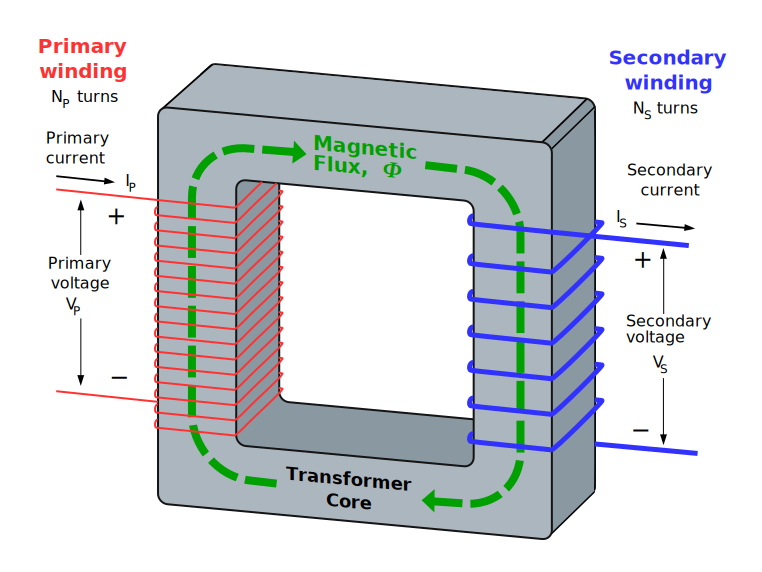
\includegraphics[width=10cm]{Transformer3d-col3}
\centering
\caption{Symbool van een 3D transformator}
\label{fig:transformator3D}
\end{figure}

Door het magnetische veld ontstaat in de tweede spoel een spanning en kan er stroom lopen door het circuit dat aan de tweede spoel gekoppeld zit. Als de primaire en de secundaire spoelen een gelijk aantal windingen hebben dan is de primaire spanning gelijk aan de secundaire spanning. Heeft de primaire spoel twee keer zoveel windingen als de secundaire spoel, dan wordt de spanning verlaagt met de helft. Dus 230 Vac aan de primaire kant wordt dan 115 Vac aan de secundaire kant. Heeft de primaire kant minder wikkelingen dan de secundaire kant dan wordt de spanning verhoogt.

De omrekening van primaire spanning naar secundaire spanning kan gedaan worden via de formule \[ V_s = V_p \frac{N_p}{N_s} \].


\chapter{Boolean Algebra}
\input{src/boolean_intro}
\section{NOT - Inverter}
\input{src/not}
\section{AND}
De AND\index{AND} geeft aan wanneer beide ingangen 1 zijn, alleen dan is de uitgang 1.

\rowcolors{2}{gray!10}{gray!20}
\begin{tabular}{ |c|c|c| }
\hline
\rowcolor{gray!60}
	Input 1 & Input 2 & Output \\
	\hline
	0 & 0 & 0 \\
	\hline
	0 & 1 & 0 \\
	\hline
	1 & 0 & 0 \\
	\hline
	1 & 1 & 1 \\
	\hline
\end{tabular}

Het symbool voor de AND is weergegeven in figuur \ref{symbool:and}

\begin{figure}[h]
\includegraphics{and_symbool}
\centering
\caption{Symbool van een AND}
\label{symbool:and}
\end{figure}

De AND wordt gebouwd door gebruik te maken van twee transistoren waarvan de beide basis de ingang vormen en een weerstand (figuur \ref{circuit:and}.

\begin{figure}[h]
\includegraphics{and_circuit}
\centering
\caption{AND circuit}
\label{circuit:and}
\end{figure}


\section{NAND}
De NAND\index{NAND} geeft een negatief resultaat als beide ingangen 1 zijn, de uitgang is dan 0.

\rowcolors{2}{gray!10}{gray!20}
\begin{tabular}{ |c|c|c| }
\hline
\rowcolor{gray!60}
	Input 1 & Input 2 & Output \\
	\hline
	0 & 0 & 1 \\
	\hline
	0 & 1 & 1 \\
	\hline
	1 & 0 & 1 \\
	\hline
	1 & 1 & 0 \\
	\hline
\end{tabular}

Het symbool voor de NAND is weergegeven in figuur \ref{symbool:nand}

\begin{figure}[h]
\includegraphics{nand_symbool}
\centering
\caption{Symbool van een NAND}
\label{symbool:nand}
\end{figure}

De NAND wordt gebouwd door gebruik te maken van twee transistoren waarvan de beide basis de ingang vormen en een weerstand (figuur \ref{circuit:nand}.

\begin{figure}[h]
\includegraphics{nand_circuit}
\centering
\caption{NAND circuit}
\label{circuit:nand}
\end{figure}

De NAND-technologie kan je tegen komen in flash memory.


\section{OR}
De OR\index{OR} geeft aan of \'e\'en of beide ingangen 1 zijn, als dat het geval is dan is de uitgang 1.

\rowcolors{2}{gray!10}{gray!20}
\begin{tabular}{ |c|c|c| }
\hline
\rowcolor{gray!60}
	Input 1 & Input 2 & Output \\
	\hline
	0 & 0 & 0 \\
	\hline
	0 & 1 & 1 \\
	\hline
	1 & 0 & 1 \\
	\hline
	1 & 1 & 1 \\
	\hline
\end{tabular}

Het symbool voor de OR is weergegeven in figuur \ref{symbool:or}

\begin{figure}[h]
\includegraphics{or_symbool}
\centering
\caption{Symbool van een OR}
\label{symbool:or}
\end{figure}

De OR wordt gebouwd door gebruik te maken van twee transistoren die parallel aan elkaar staan, de beide basis vormen de ingang en er is een weerstand (figuur \ref{circuit:or}.

\begin{figure}[h]
\includegraphics{or_circuit}
\centering
\caption{OR circuit}
\label{circuit:or}
\end{figure}


\section{NOR}
De NOR\index{NOR} geeft aan dat beide ingangen 0 zijn, als dat het geval is dan is de uitgang 1.

\rowcolors{2}{gray!10}{gray!20}
\begin{tabular}{ |c|c|c| }
\hline
\rowcolor{gray!60}
	Input 1 & Input 2 & Output \\
	\hline
	0 & 0 & 1 \\
	\hline
	0 & 1 & 0 \\
	\hline
	1 & 0 & 0 \\
	\hline
	1 & 1 & 0 \\
	\hline
\end{tabular}

Het symbool voor de NOR is weergegeven in figuur \ref{symbool:nor}

\begin{figure}[h]
\includegraphics{nor_symbool}
\centering
\caption{Symbool van een NOR}
\label{symbool:nor}
\end{figure}

De NOR wordt gebouwd door gebruik te maken van twee transistoren die parallel aan elkaar staan, de beide basis vormen de ingang en er is een weerstand (figuur \ref{circuit:nor}.

\begin{figure}[h]
\includegraphics{nor_circuit}
\centering
\caption{NOR circuit}
\label{circuit:nor}
\end{figure}


\section{XOR}
\input{src/xor}
\section{XNOR}
De XNOR\index{XNOR} geeft als \'e\'en van beide ingangen 1 is en de andere 0 een 0 op de uitgang.

\rowcolors{2}{gray!10}{gray!20}
\begin{tabular}{ |c|c|c| }
\hline
\rowcolor{gray!60}
	Input 1 & Input 2 & Output \\
	\hline
	0 & 0 & 1 \\
	\hline
	0 & 1 & 0 \\
	\hline
	1 & 0 & 0 \\
	\hline
	1 & 1 & 1 \\
	\hline
\end{tabular}

Het symbool voor de XNOR is weergegeven in figuur \ref{symbool:xnor}

\begin{figure}[h]
\includegraphics{xnor_symbool}
\centering
\caption{Symbool van een XNOR}
\label{symbool:xnor}
\end{figure}

Er zijn vele manieren om een XNOR te bouwen, er is dan ook geen circuit opgenomen. Zie Wikipedia voor mogelijke oplossingen.



%%%%%%%%%%%%%%%%%%%%%
%%% Index and End %%%
%%%%%%%%%%%%%%%%%%%%%
\backmatter
\printindex
\end{document}

%%% Last line %%%
